\documentclass[doc,natbib]{apa6}

\usepackage{graphicx}
\usepackage{multicol}
\usepackage{float}
\usepackage{hyperref}
\usepackage{tabularx}
\usepackage{array}
\usepackage{pgfgantt}
\usepackage{rotating}
\raggedbottom

\title{Smart City Visualisation: Interactive Data Visualisation for New York Taxi Operational Data}
\author{Qiru Wang}
\affiliation{\href{mailto:689404@swansea.ac.uk}{689404@swansea.ac.uk} \\ Department of Science \\ Swansea University, Wales UK}
\abstract{To be abstracted}
\shorttitle{Smart City Visualisation}
\begin{document}
\maketitle
\setlength{\parindent}{0pt}
\setlength{\parskip}{0.8em}
\newpage
\tableofcontents
\newpage
\setcounter{secnumdepth}{5}
\section{Introduction}

The rapid expansion of cities mandates the implantation of Smart City, the definition of Smart City may vary from country to country, but the common interest behind is to improve life quality of its citizens by the optimisation of current resources \citep{Lazaroiu2012}, to mitigate the problems produced by rapid growth of population (including ageing population) and rapid urbanisation \citep{Chourabi2011}. In every city, operational data of the city is being collected via Information and Communication Technology (ICT) \citep{Deakin2011}, while investing insufficient effort into gathering useful insights and knowledge that the data holds. One of the reasons behind is that raw data is laborious to analyse with human eyes, without effective data visualisation techniques, which extracts the meaningful information by transforming raw data into graphical representations that convey more information via human visual cognition \citep{Ward2010}. 

Since sight is one of our key senses for information understanding, the initiative of this project is to develop an interactive visualisation toolset, revealing the meaningful insights underlie the taxi operational data in New York, collected by New York City Taxi \& Limousine Commission, in conjunction with real-time traffic monitoring data provided by Mapbox. The toolset will be beneficial to users across different levels.

The toolset will enable users to dynamically explore, analyse and present the dataset imported, whether it is multivariate, geospatial or time-oriented. The performance of this toolset will be a key benchmark for its success, the target is to deliver a smooth and lightweight toolset with cross-platform compatibility, thus the form of Web Application is chosen. During the planning phase, the existing tools will be reviewed to find out their advantages and disadvantages, and those will be thoroughly considered for development.

One challenge faced in this project will be the data itself. Having different data source providers will result in different data formats, that often require tedious process for pre-processing. In order to overcome that, a Java program will be written specifically for pre-processing data into JSON format, which is both human readable and program friendly. Another challenge will be the tight schedule, some trade-off in interface design will be made in order to ensure the delivery of functionalities.

\hyperref[sec2]{Section 2 Background} introduces the background of Smart City, Data Visualisation and the relationships between two topics. In this section, a literature review of related research is also conducted along with experimenting existing tools for visualisation. A subsection of Data Characteristics [change to hyperlink] describes the taxi operational data and real-time traffic monitoring data.

\hyperref[sec3]{Section 3 Project Specification} includes the functionalities set to be delivered by the end of this project, and a specification for programming languages used during this project. \hyperref[sec4]{Section 4 Project Plan and Timetable} includes a Gantt chart of this project.\hyperref[sec5]{Section 6 Initial Implementation} describes the steps to pre-process the taxi dataset along with the basic functionalities provided by the toolset.

\section{Background}
\label{sec2}
The definition of Smart City has been adapting over the decades, the fundamentals of Smart City is to improve a city's efficiency sustainably \citep{Caragliu2011}, thus improving the life quality of its citizens. To achieve sustainability means the optimisation of current resources is critical, by:
\begin{itemize}
	\item Collecting operational data of the city via Information and Communication Technology (ICT) \citep{Deakin2011}
	\item Pre-processing the raw data into suitable formats
	\item Harvesting useful information via data analysis
	\item Policy-making base on the analytical results \citep{Lazaroiu2012}
\end{itemize}
In order to carry out effective data analysis, the data collected has to be rigorously pre-processed and visualisations should be generated to convey the underlie information. This further requires appropriate Data Visualisation techniques.

\subsection{Related Work}
This section reviews related work in the field of Smart City and Data Visualisation.\hfil\newline

\subsubsection{Understanding Smart Cities: An Integrative Framework}\hfil\newline
Understand Smart Cities \citep{Chourabi2011} is a comprehensive paper about smart city. The paper discusses the motivations and purposes behind smart city and gives a set of working definitions of a smart city, a city that monitors and connects its physical infrastructures with ICTs to leverage the efficiency, sustainability, equitability and liveability of the city. 

The paper describes a framework with eight crucial factors of a successful smart city:
\begin{multicols}{2}
	
	\begin{itemize}
		\item Management and organisation
		\item Technology
		\item Governance
		\item Policy
		\item People and communities
		\item Economy
		\item Build infrastructure
		\item Natural environment
	\end{itemize}
\end{multicols}
For each of the eight factors, authors detail the challenges faced and the possible strategies to counter them. In particular, the paper emphasises that the inclusions of complex analytics to make better policies, requires visualisation techniques in the decision-making process.

Authors acknowledge that the capture of data from various ICT infrastructures is key to a successful smart city, the decisions made upon those data acquired will offer huge potentials in optimising the operation of the city.

By gaining deep understanding of what a smart city is, this paper inspires the development of this project, precisely what the requirement specification of visualisation tool that suites the needs of smart city.

\subsubsection{Interactive Data Visualization: Foundations, Techniques, and Applications}\hfil\newline
Interactive Data Visualization is a book \citep{Ward2010} introducing the fundamentals of data visualisation concepts and techniques. The book covers the spectrum of usage for data visualisation across different industries.

The book defines visualisation as ``the communication of information using graphical representations'', the use of data visualisation techniques is prominent to convey more information underlie the dataset given via human visual cognition system. As mentioned by authors in the book, human as visual beings, absorbing information contained in graphs is more efficient than in text or in other formats \citep[pp. 3-5]{Ward2010}.

\begin{figure}[H]
	\centering
	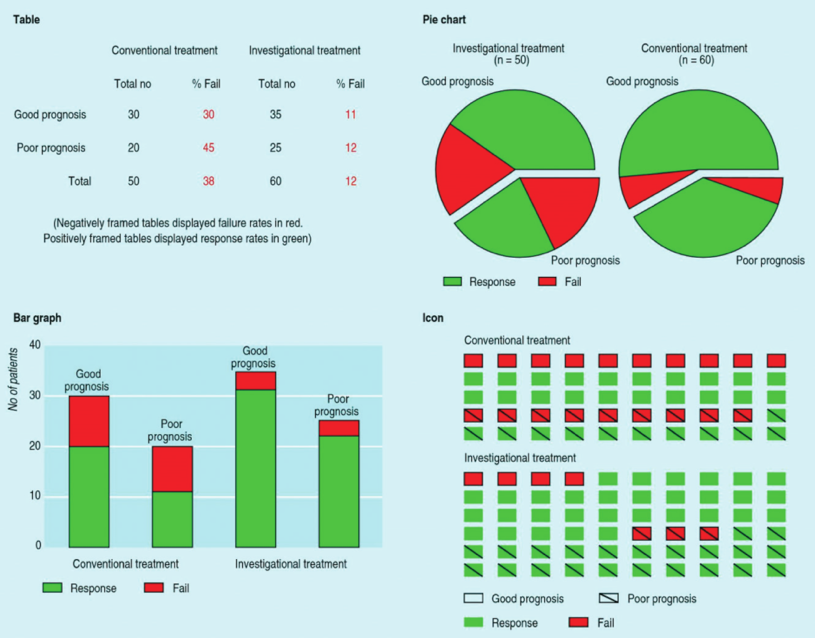
\includegraphics{figures/fig1.png}
	\caption{\label{fig:1}Examples of the four types of display of hypothetical clinical trial data \citep{Elting1999}}
\end{figure}

Data visualisation also plays an important role in the decision-making process. The same data presented in different visualisations will have different impact on the final decision. In Figure \ref{fig:1}. is the study conducted by \citeauthor{Elting1999} \citep{Elting1999} on the influence of visualisation types on clinical decisions, it uses a table, a stacked bar graph, a pie chart and an icon display showing exactly the same dataset, the results of a clinical trial from both conventional and investigational treatments. When a specially chosen group of competent physicians were asked to make a decision whether the clinical trial should be stopped or not, their decision accuracies were interestingly fluctuating from four visualisations, as seen in Table \ref{tab:1}.

\begin{table}[H]
	\centering
			\caption{Performance on four types of visualisation in the study conducted \citep{Elting1999}}
	\label{tab:1}
	\begin{tabularx}{\textwidth}{p{3.7cm}>{\raggedleft\arraybackslash} p{2.8cm}>{\raggedleft\arraybackslash} p{3.6cm}>{\raggedleft\arraybackslash} X}
		\hline\hline
		\textbf{Visualisation Type} & \textbf{Decision Time} & \textbf{Decision Accuracy} & \textbf{Preference Rate} \\\hline
		Table                       & 35 seconds             & 68\%                       & 61.7\%                   \\
				Stacked bar graph           & 34 seconds             & 43\%                       & 23.5\%                   \\
		Pie chart                   & 36 seconds             & 56\%                       & 14.8\%                   \\
		Icon display                & 37 seconds             & 82\%                       & 0\%                      \\\hline
		\hline
	\end{tabularx}
\end{table}

Despite having the highest decision accuracy with similar time taken for making the decision, icon display was not preferred by any of the participants.
Apart from the foundations of data visualisation, there are three chapters that are particularly valuable for this project: 

\begin{itemize}
	\item Visualization Techniques for Geospatial Data
	\item Visualization Techniques for Time-Oriented Data
	\item Visualization Techniques for Multivariate Data 
\end{itemize}

In each chapter, not only that authors present the techniques for visualisations, but also list down the issues faced during visualising the data. Since the proposed toolset that will be mainly used for visualising those three types of data, this book is then extremely beneficial to the development.

\paragraph{Visualization Techniques for Geospatial Data}\hfill\\
One of the planned visualizations will be to visualise the origin and destination of taxi dataset on a geographic flow map with interactive features. However, the points are often clustering together as shown in Figure \ref{fig:2}, in order to generate a geographic flow map that effectively conveys meaningful message, in this chapter authors suggest that those points should be generalised. The process of generalisation involves simplifying points, which essentially means removing or combining the points that are not separately visible on a map with suitable scale \citep[pp. 247-249]{Ward2010}.

\begin{figure}[H]
	\centering
	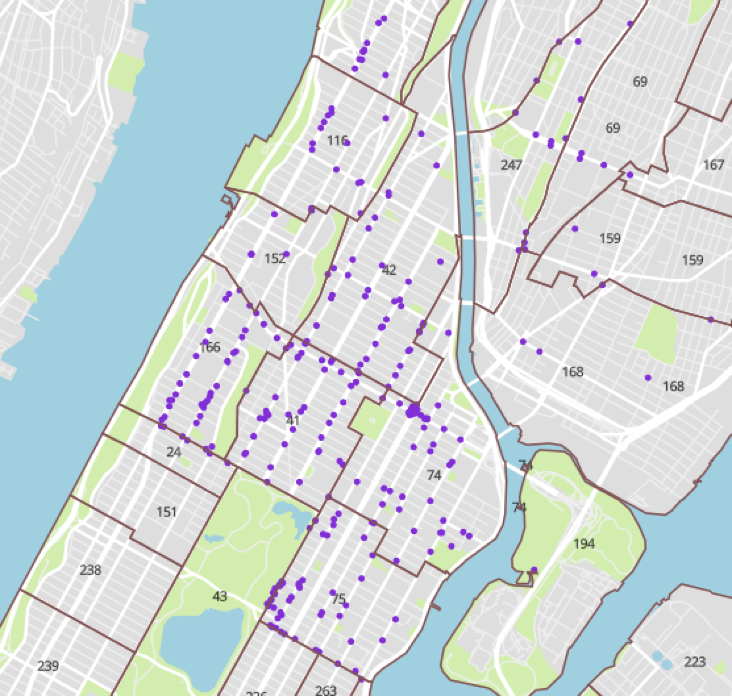
\includegraphics{figures/fig2.png}
	\caption{\label{fig:2}Visualisation of taxi pick-up locations in New York on a prototype of the proposed toolset using Mapbox \citep{Mapbox2017}}
\end{figure}

\paragraph{Visualization Techniques for Time-Oriented Data}\label{par:Visualization Techniques for Time-Oriented Data}\hfill\\
According to the authors, time itself is a dimension of any dataset with distinct characteristics, the importance of revealing patterns and relationships of time dimension with other dimensions is illustrated in this chapter. \citep[p. 254]{Ward2010}.

Figure \ref{fig:3} below shows the visualisations of one time-oriented dataset for cases of influenza occurred daily in Germany in a period of three years. The left visualisation is a simple line lot to linearly visualise the data, it clearly shows the peak times of influenza occurrence but the patterns underlie the dataset is hard to conclude. The centre (with one cycle represents 24 days) and the right (with one cycle represents 28 days) use a cyclic visualisation which utilises a spiral-shaped time axis. 

There is no pattern to be recognised in the centre visualisation. By adjusting the cycle length to fit into the data's natural interval (multiple of 7 days), the right visualisation is obtained, which instantly reveals that more influenza cases occurred in Mondays than any other days. This example demonstrates that the characteristics of time can significantly change ``the expressiveness of visual representations'' \citep[p. 254]{Ward2010}.

\begin{figure}[H]
	\centering
	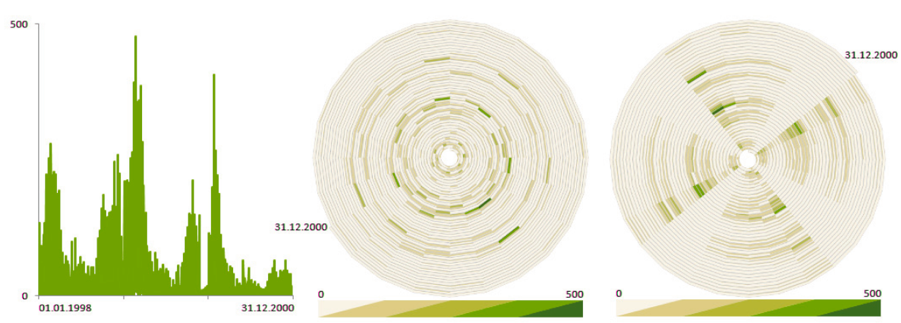
\includegraphics{figures/fig3.png}
	\caption{\label{fig:3}Linear vs cyclic visualisation of time-oriented data \citep[p. 255]{Ward2010}}
\end{figure}

For the taxi dataset used for this project, discrete time data is introduced in multiple fields, e.g. taxi pick up time and drop off time. According to the authors, discrete time data is the most widely used quantitative time model. Such dataset can be studied to find out the hidden patterns and 3D visualisation often provides better illustration of time-oriented dataset \citep[pp. 258-263]{Ward2010}.

\paragraph{Visualization Techniques for Multivariate Data}\hfil\\
In the field of Data Visualisation, multivariate data refers to datasets that have more than three variables. Visualisation of multivariate data is referred by Liu \citep{Liu} as \textit{Curse of Dimension} due to the fact that the effectiveness of retinal visual elements such as colour, shape and size will deteriorate as the number of variables increases.

This chapter introduces visualisation techniques that maintain characteristics of multivariate dataset while providing effective renderings. The taxi dataset contains multiple point plots as the main data format, therefore the techniques for visualising point-based multivariate data is beneficial to the development of the proposed toolset. Four point-based techniques are described \citep[pp. 285-292]{Ward2010} in this chapter as follows:

\begin{itemize}
	\item Dimension Subsetting -- dimensions can be selectively displayed by the user or the toolset automatically selects the most meaningful dimensions to visualise.
	\item Dimension Reduction -- dimensionality reduction algorithms such as principal component analysis (PCA) will be applied to project higher dimensional dataset into lower dimensions, meanwhile it tries to reduce the loss of information to the minimal during the process.
	\item Dimension Embedding -- dimensions can be mapped to many graphical representations besides position, e.g. colour, size and shape. This is however limited as mentioned previously as \textit{Curse of Dimension}.
	\item Multiple Displays -- visualisations are superimposed or juxtaposed. The classic example of multiple displays is the use of scatterplot matrix.
\end{itemize}

\subsection{Existing Software API}
\subsubsection{AnyMap.js}\hfil\newline
AnyMap.js is a JavaScript based geospatial visualisation library that was initially written for businesses who want to transform operational data into actionable information via data visualisation. The library requires a commercial license but it is available for personal evaluation for an unlimited period of time here: \url{https://static.anychart.com/cdn/js/7.13.1/anymap.min.js?download}. 

It provides great cross-platform compatibility with support for popular data formats such as XML and JSON. AnyMap.js is also embedded with a full set of JavaScript API and offers a variety of options to create geospatial visualization with interactivity and simplicity.

Figure \ref{fig:4}, Figure \ref{fig:6} and Figure \ref{fig:5} are examples of Bubble Map,Connector Map and Choropleth Map that are enlightening for the development of this proposed toolset.

\begin{figure}[H]
	\centering
	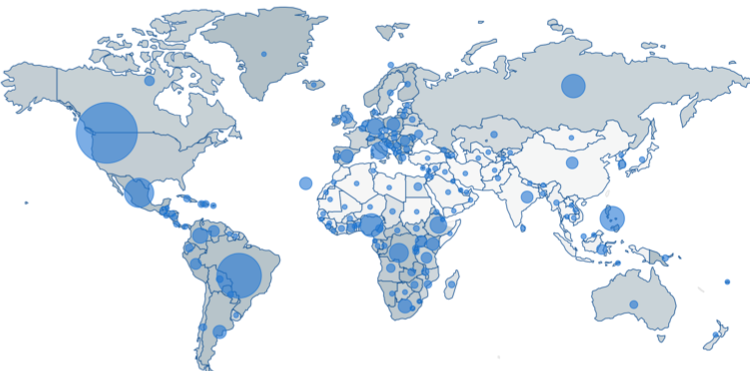
\includegraphics[height=6.3cm,keepaspectratio]{figures/fig4.png}
	\caption{\label{fig:4}Visualisation using a Bubble Map with AnyMap.js \citep{AnyChart2017a}}
\end{figure}

\begin{figure}[H]
	\centering
	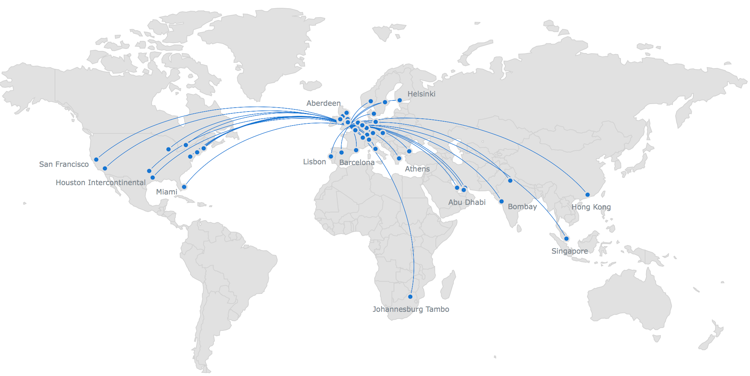
\includegraphics[height=6.3cm,keepaspectratio]{figures/fig6.png}
	\caption{\label{fig:6}Visualisation using a Connector Map with AnyMap.js \citep{AnyChart2017}}
\end{figure}

\begin{figure}[H]
	\centering
	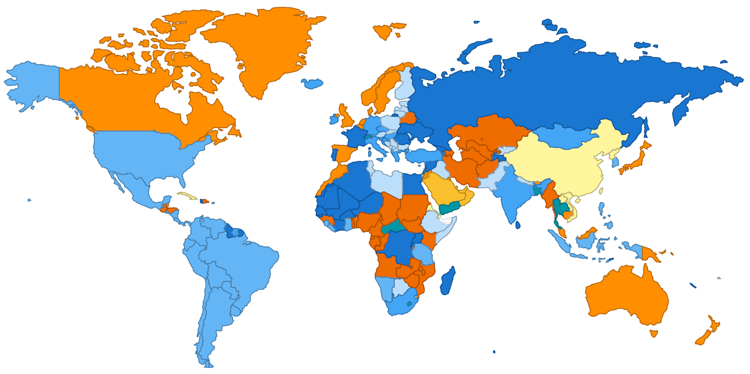
\includegraphics[height=6.3cm,keepaspectratio]{figures/fig5.png}
	\caption{\label{fig:5}Visualisation using a Choropleth Map with AnyMap.js  \citep{AnyChart2017b}}
\end{figure}

\subsubsection{Mapbox Studio and Mapbox.js}\hfil\newline
Mapbox is mapping platform for developers. Mapbox Studio is a web application that enables developers to create base map style with ease. It allows the user to upload geospatial dataset in GeoJSON and CVS format, Mapbox Studio will then convert the dataset into a format called Tileset that stores both vector and raster data. Each tileset can be visualised on a base map as a separated layer. By doing this, a map can be modified to visualise arbitrary dimensions of data. 

In Figure \ref{fig:7} below, six customised layers are visualised on a base map of New York.
\begin{enumerate}
	\item Taxi zones are segmented using brown boundary.
	\item Taxi pick-up locations are depicted using purple dots.
	\item Low traffic congestion is mapped to lines in green.
	\item Moderate traffic congestion is mapped to lines in yellow.
	\item Heavy traffic congestion is mapped to lines in orange.
	\item Severe traffic congestion is mapped to lines in red.
\end{enumerate}

Those layers form a new base map and Mapbox Studio outputs a unique URL of that base map. By making API request containing the unique URL using Mapbox.js, the newly created base map can be initialised on different platforms as long as JavaScript and HTML are supported.

\begin{figure}[H]
	\centering
	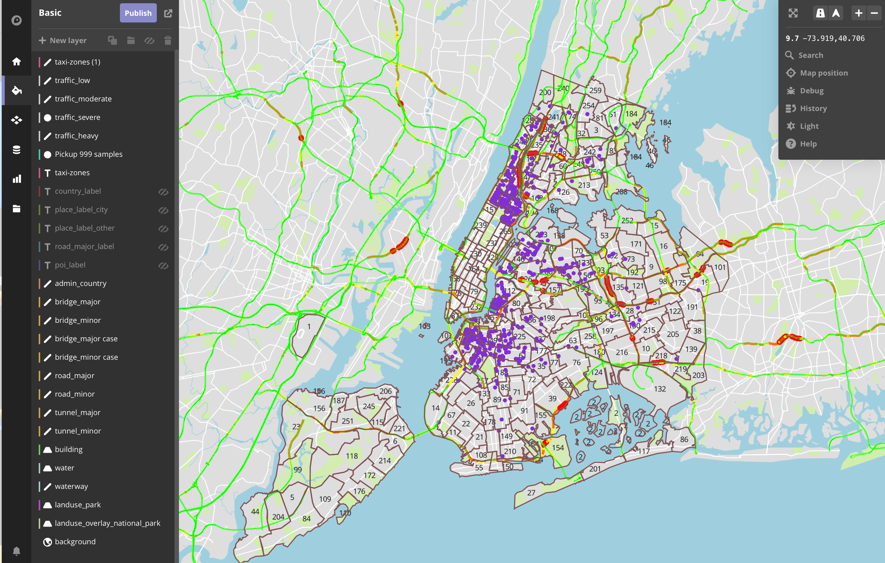
\includegraphics{figures/fig7.png}
	\caption{\label{fig:7}Interface of Mapbox Studio when creating a prototype base map \citep{Mapbox2017}}
\end{figure}

\subsection{Similar Applications}
\subsubsection{MONiTOUR}\label{sec:monitour}\hfil\newline
MONiTOUR \citep{SenseableCityLab-Ewaste} in Figure \ref{fig:8}, is an e-waste tracker that visualises the travel routes of obsoleted printers, LCD and CRT monitors from the US. As a part of the joint project \textit{e-trash Transparency Project}, MIT Senseable City Lab and Basel Action Network embedded GPS trackers into those e-wastes in order to obtain the travel routes. 

The results are visualised on a world map, blue dots and read dots represent origin and destination respectively, with white lines clear depict that the majority of e-waste travelled to Asia. Filtering on device type and region. Figure \ref{fig:9} shows when a route is selected, the detailed travel history of the GPS tracker in steps. 

The app is written in JavaScript with HTML 5 and the base map is from Mapbox, it is available for free at \url{http://senseable.mit.edu/monitour-app/}

\begin{figure}[H]
	\centering
	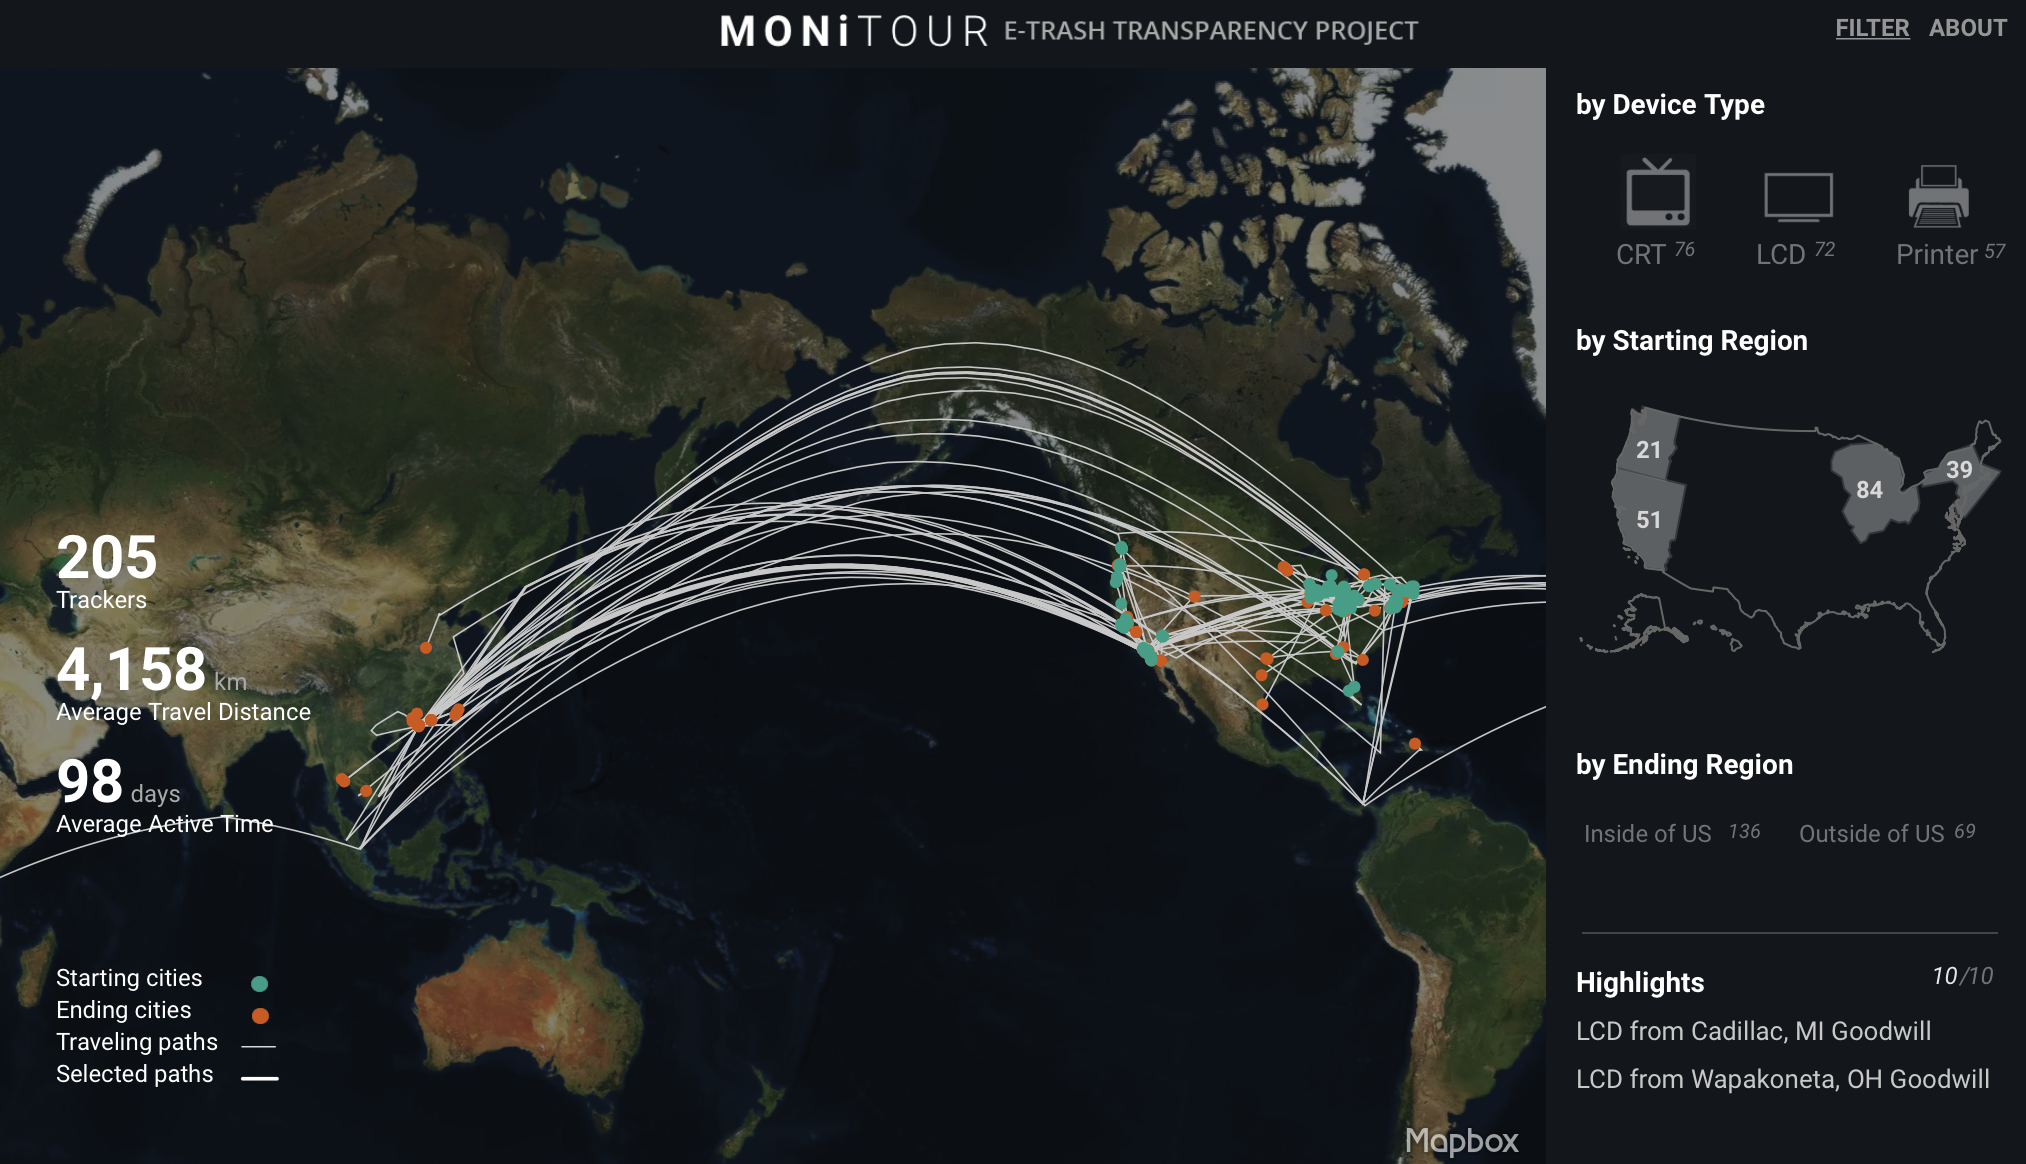
\includegraphics[width=\textwidth,keepaspectratio]{figures/fig8.png}
	\caption{\label{fig:8}Interface of MONiTOUR visualising origins, destinations and paths of 205 GPS trackers embedded into printers, LCD and CRT monitors \citep{SenseableCityLab-Ewaste}.}
\end{figure}

\begin{figure}[H]
	\centering
	\includegraphics[width=\textwidth,keepaspectratio]{figures/fig9.png}
	\caption{\label{fig:9}Interface of MONiTOUR visualising the travel history of a GPS tracker embedded into a LCD monitor, from Seattle to Hong Kong \citep{SenseableCityLab-Seattle}.}
\end{figure}

\subsubsection{Boston 311}\label{sec:boston311}\hfil\newline
Boston 311 \citep{Boston311} in Figure \ref{fig:10} is a geospatial visualisation of 3-1-1 incident reports in Boston from October 2010 to June 2012. 
\begin{figure}[H]
	\centering
	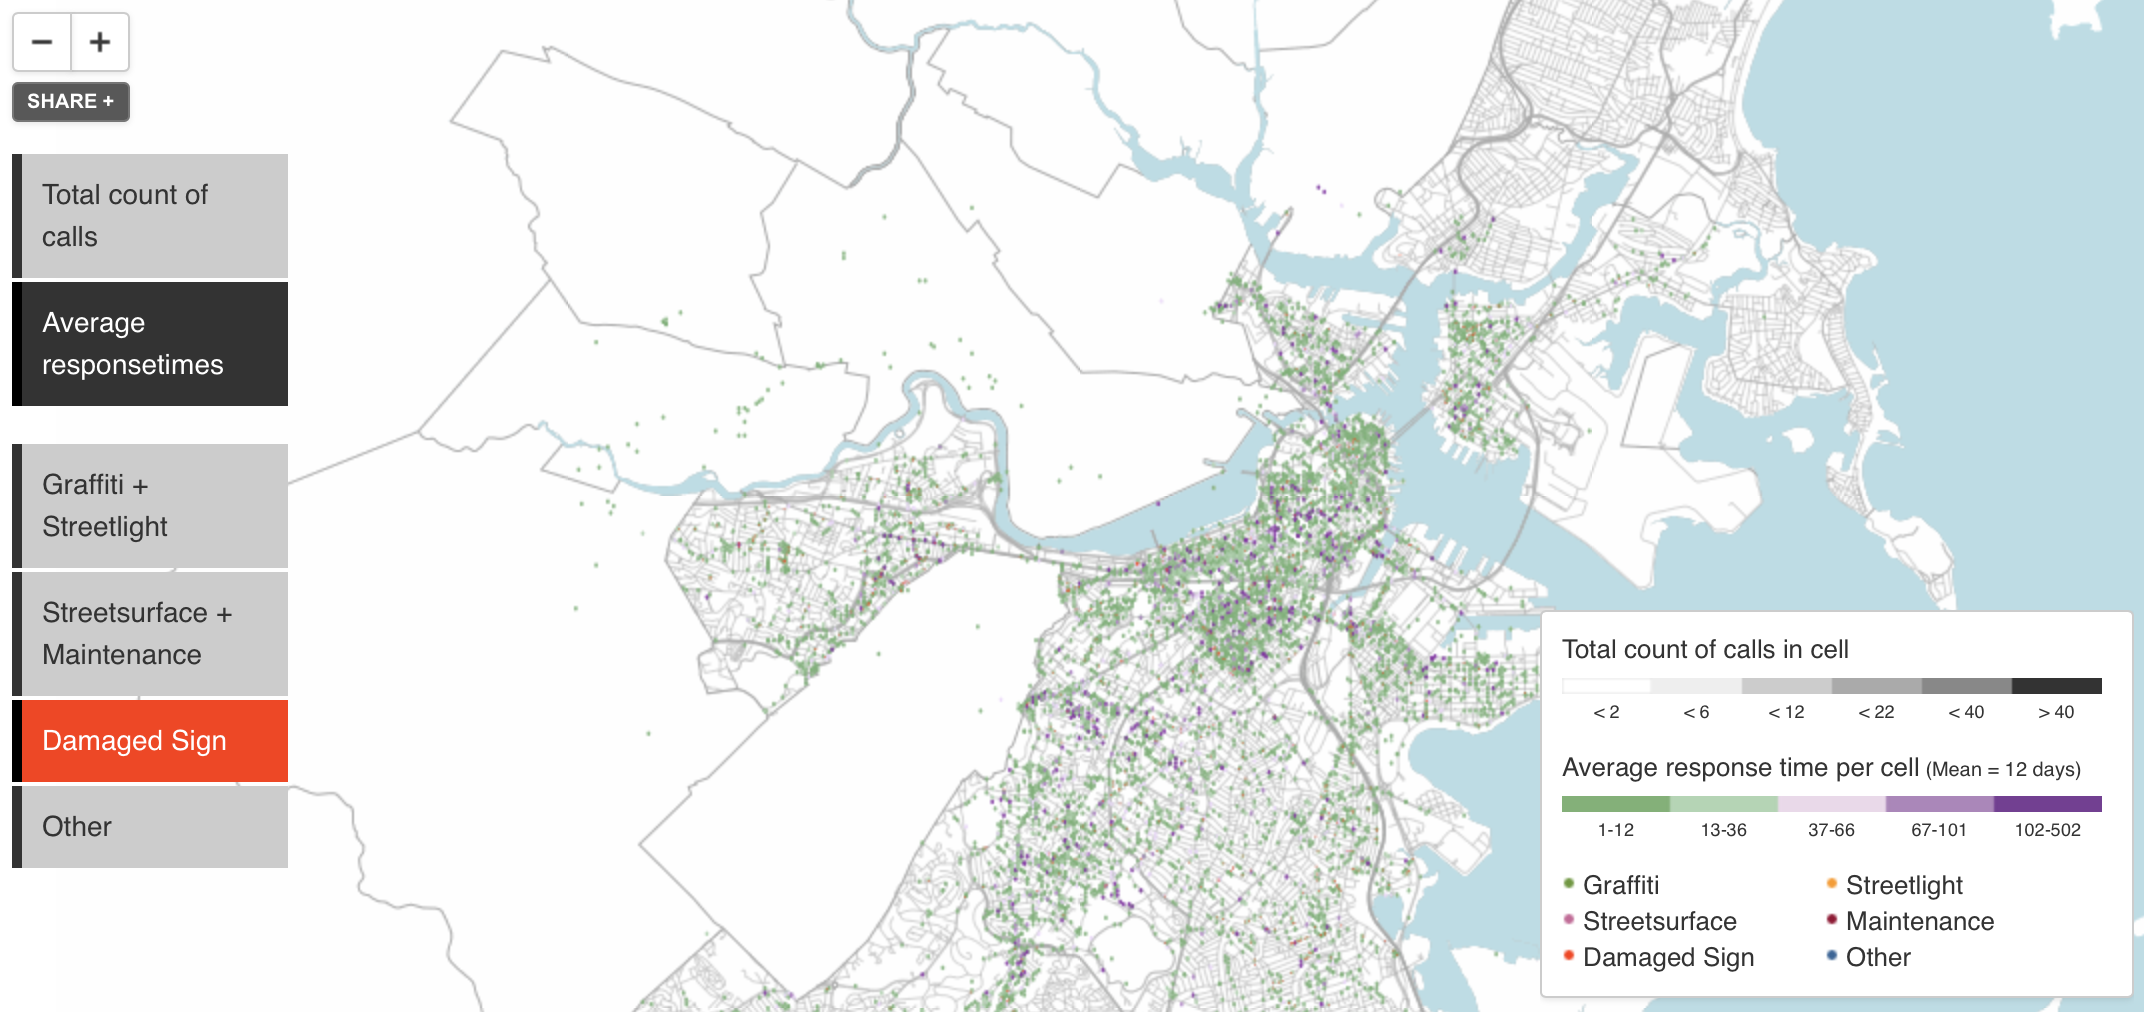
\includegraphics[width=\textwidth,keepaspectratio]{figures/fig10.png}
	\caption{\label{fig:10}Interface of Boston311 visualising average response time against damaged sign in Boston \citep{Boston311}.}
\end{figure}

Two dimensions can be visualised simultaneously by selecting them on the left panel. The first dimension can be either total count of calls or average response time, whereas the second dimension can be chosen from graffiti and streetlight, streetsurface and maintenance, damaged sign or other.

\subsection{Limitation of Similar Applications}
Both \hyperref[sec:monitour]{MONiTOUR} and \hyperref[sec:boston311]{Boston 311} pose limitations on visualising taxi operational data. 

\subsubsection{MONiTOUR}\hfil\newline
The performance of MONiTOUR is a major concern for visualisation of millions of taxi operational data entries. During the experiment of MONiTOUR, even there are only 205 distinct paths visualised on the map, the performance is not optimal. The web app lags significantly when applying zoom and pan operations, using Chrome (Version 58.0.3029), Firefox (Version 52.1.0) and Safari (Version 10.1). The initialisation of the application also takes more than ten seconds with fast internet connection.

Certain level of filtering is allowed in MONiTOUR but is far from sufficient for visualisation of taxi operational data, due to the high dimensionality.

Visualisation of time-oriented data is not built into this application.

\subsubsection{Boston 311}\hfil\newline
Boston 311 successfully visualises high volume of data with satisfactory performance. However, a generalisation process mentioned in \hyperref[par:Visualization Techniques for Time-Oriented Data]{Section \textit{Visualization Techniques for Time-Oriented Data}} is missing and causes data points to be clustered and overlapping each other regardless of zoom level. This creates confusions during presentation stage to users. 

Filtering is extremely limited in Boston 311, apart from selecting different dataset, users are unable to select subset of data for visualisation.

Visualisation of time-oriented data is not built into this application.

\subsection{Data Characteristics}
\subsubsection{Taxi Operational Data recorded by the New York City Taxi \& Limousine Commission (TLC)}\hfil\newline
Taxicab \& Livery Passenger Enhancement Programs (TPEP/LPEP) was introduced in March 2004 by the TLC, the primary objective this program is to improve New York taxi service by implementing specific technology to collect taxi operational data, including pick-up and drop-off location, trip distance and time, passenger counts and others. Prior to the TPEP/LPEP, this data collection process was manually done by the drivers using a hand-written log book, the introduction of the program significantly improved accuracy of the data and efficiency of the data collection process \citep{NYCTaxi&LimousineCommission}.

Table \ref{tab:2} shows the description of the data provided by TLC at \url{http://www.nyc.gov/html/tlc/html/about/trip_record_data.shtml}.

For each month, three datasets in CSV format are provided, Yellow Taxi, Green Taxi and For-hire Vehicle (FHV). Due to the nature of FHV service, its dataset contains only pick-up time and pick-up borough ID, thus the dataset is not used in this project.

Table \ref{tab:3} shows the difference between three datasets in terms of dataset size and number of records. 

\begin{table}[H]
	\centering
			\caption{Taxi operational datasets \citep{NYCTaxi&LimousineCommission2017}. Each month the size and number of records vary slightly, all data shown in the table are estimated average.}
	\label{tab:3}
	\begin{tabularx}{\textwidth}{X >{\raggedleft\arraybackslash}X >{\raggedleft\arraybackslash}X}
		\hline\hline
		\textbf{Dataset} & \textbf{Dataset size} & \textbf{Number of records} \\
		Yellow Taxi                       & 1800 MB             & 11,500,000                   \\
		Green Taxi           & 200 MB             & 1,500,000                 \\
		For-Hire Vehicle (FHV)                   & 300 MB        &     8,500,000                  \\\hline
		\hline
	\end{tabularx}
\end{table}

\begin{table}[H]
\caption{Description of taxi operational data collected by TLC \citep{NYCTaxi&LimousineCommission2015}.}
\label{tab:2}
	\centering
	\begin{tabularx}{\textwidth}{p{4cm}|p{2.1cm}|X|>{\raggedleft\arraybackslash}p{2.1cm}}
		\hline\hline
		\textbf{Column Name}    & \textbf{Data Type} & \textbf{Data Description}                                                                                                                                     & \textbf{Sample}  \\\hline
		VendorID                & Integer            & Vendor that provided the data \newline 1= Creative Mobile Technologies, LLC \newline 2= VeriFone Inc.                                                                                                                                                       & 1                \\\hline
		Lpep\_pickup\_datetime  & Datetime           & Taxi pick-up date time                                                                                                                                         & 01/01/2015 02:21 \\\hline
		Lpep\_dropoff\_datetime & Datetime           & Taxi drop-off date time                                                                                                                                        & 01/01/2015 03:21 \\\hline
		RateCodeID              & Integer            & Rate code for the trip \newline 1= Standard rate \newline 2=JFK \newline 3=Newark\newline 4=Nassau or Westchester \newline  5=Negotiated fare \newline 6=Group ride                                                                                                                                                     & 1                \\\hline
		Pickup\_longitude       & Longitude          & Taxi pick-up longitude                                                                                                                                         & -73.86389923     \\\hline
		Pickup\_latitude        & Latitude           & Taxi pick-up latitude                                                                                                                                          & 40.72250748      \\\hline
		Dropoff\_longitude      & Longitude          & Taxi drop-off longitude                                                                                                                                        & -73.94389923     \\\hline
		Dropoff\_latitude       & Latitude           & Taxi drop-off latitude                                                                                                                                         & 40.70850748      \\\hline
		Passenger\_count        & Integer            & Number of passengers for the trip                                                                                                                             & 5                \\\hline
		Trip\_distance          & Double             & Total distance for the trip                                                                                                                                   & 14.01            \\\hline
		Fare\_amount            & Double             & Total fare for the trip                                                                                                                                       & 16.55            \\\hline
		Extra                   & Double             & Extra surcharge for the trip                                                                                                                                  & 0.5              \\\hline
		MTA\_tax                & Double             & Metropolitan Transit Authority Tax for the trip                                                                                                               & 0.5              \\\hline
		Tip\_amount             & Double             & Total tip amount for the trip                                                                                                                                 & 3.5              \\\hline
		Tolls\_amount           & Double             & Total toll amount for the trip                                                                                                                                & 5.33             \\\hline
		Improvement\_surcharge  & Double             & Taxi Improvement Fund surcharge                                                                                                                               & 0.3              \\\hline
		Total\_amount           & Double             & Total charge amount for the trip (Fare + all surcharges)                                                                                                             & 20.55            \\\hline
		Payment\_type           & Integer            & Payment type used for the trip \newline 1= Credit card \newline 2= Cash \newline 3= No charge \newline 4= Dispute \newline 5= Unknown \newline 6= Voided trip & 1                \\\hline
		\hline
	\end{tabularx}
\end{table}


Starting from July 2016, instead of the coordinates, only pick-up and drop-off borough ID are provided, as the result only data prior to that are used in this project. Figure \ref{fig:11} and Figure \ref{fig:12} are screenshots of Green taxi operational dataset from January 2015.

The dataset contains both geospatial (longitude and latitude) and discrete time-oriented data (pick-up and drop-off time).

\begin{figure}[H]
	\centering
	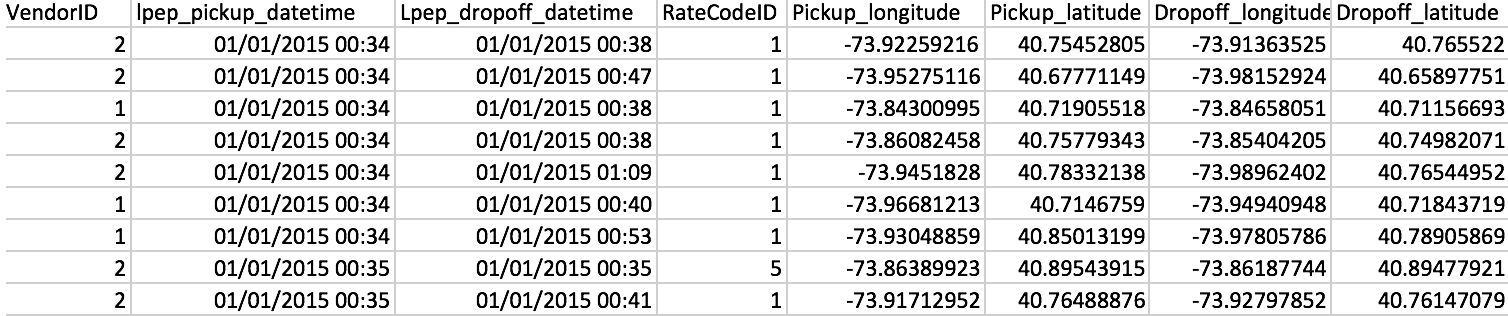
\includegraphics[width=\textwidth,keepaspectratio]{figures/fig11.png}
	\caption{\label{fig:11}Partial screenshot of Green Taxi operational dataset from January 2015 \citep{NYCTaxi&LimousineCommission2017}.}
\end{figure}

\begin{figure}[H]
	\centering
	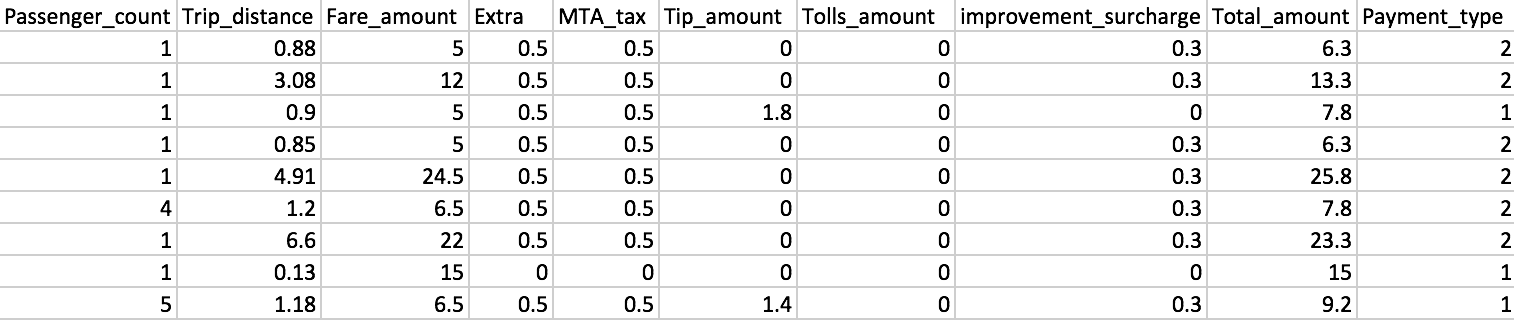
\includegraphics[width=\textwidth,keepaspectratio]{figures/fig12.png}
	\caption{\label{fig:12}Partial screenshot of Green Taxi operational dataset from January 2015 \citep{NYCTaxi&LimousineCommission2017}.}
\end{figure}

\section{Project Specification}
\label{sec3}

The primary objectives of this project is to develop a visualisation toolset for the taxi operational data. The toolset should contain the following major features:
\begin{itemize}
	\item Converting large chunk of taxi operational data in CSV format into JSON and GeoJSON formats, to be used for different software APIs
	\item Exploring the data via various types of visualisation
	\item Analysing the visualisation via different interactive functions such as filtering of data dimension or volume. 
\end{itemize}

The project should help the author to gain deeper understanding of information visualisation, the usefulness and the difficulties in obtaining such visualisation. Due to the massive amount of data used, data pre-processing will also be focused during the development phase.

\subsection{Feature Specification}
The proposed toolset will have the following features
\begin{enumerate}
	\item An interactive and responsive web application that contains
	\begin{enumerate}
	\item A tool to generate a map that predominantly as a geospatial visualisation but also contains time-oriented dimension
	\item A tool to generate a chord diagram for taxi trip origin and destination visualisation, see Figure \ref{fig:13}

\begin{figure}[H]
	\centering
	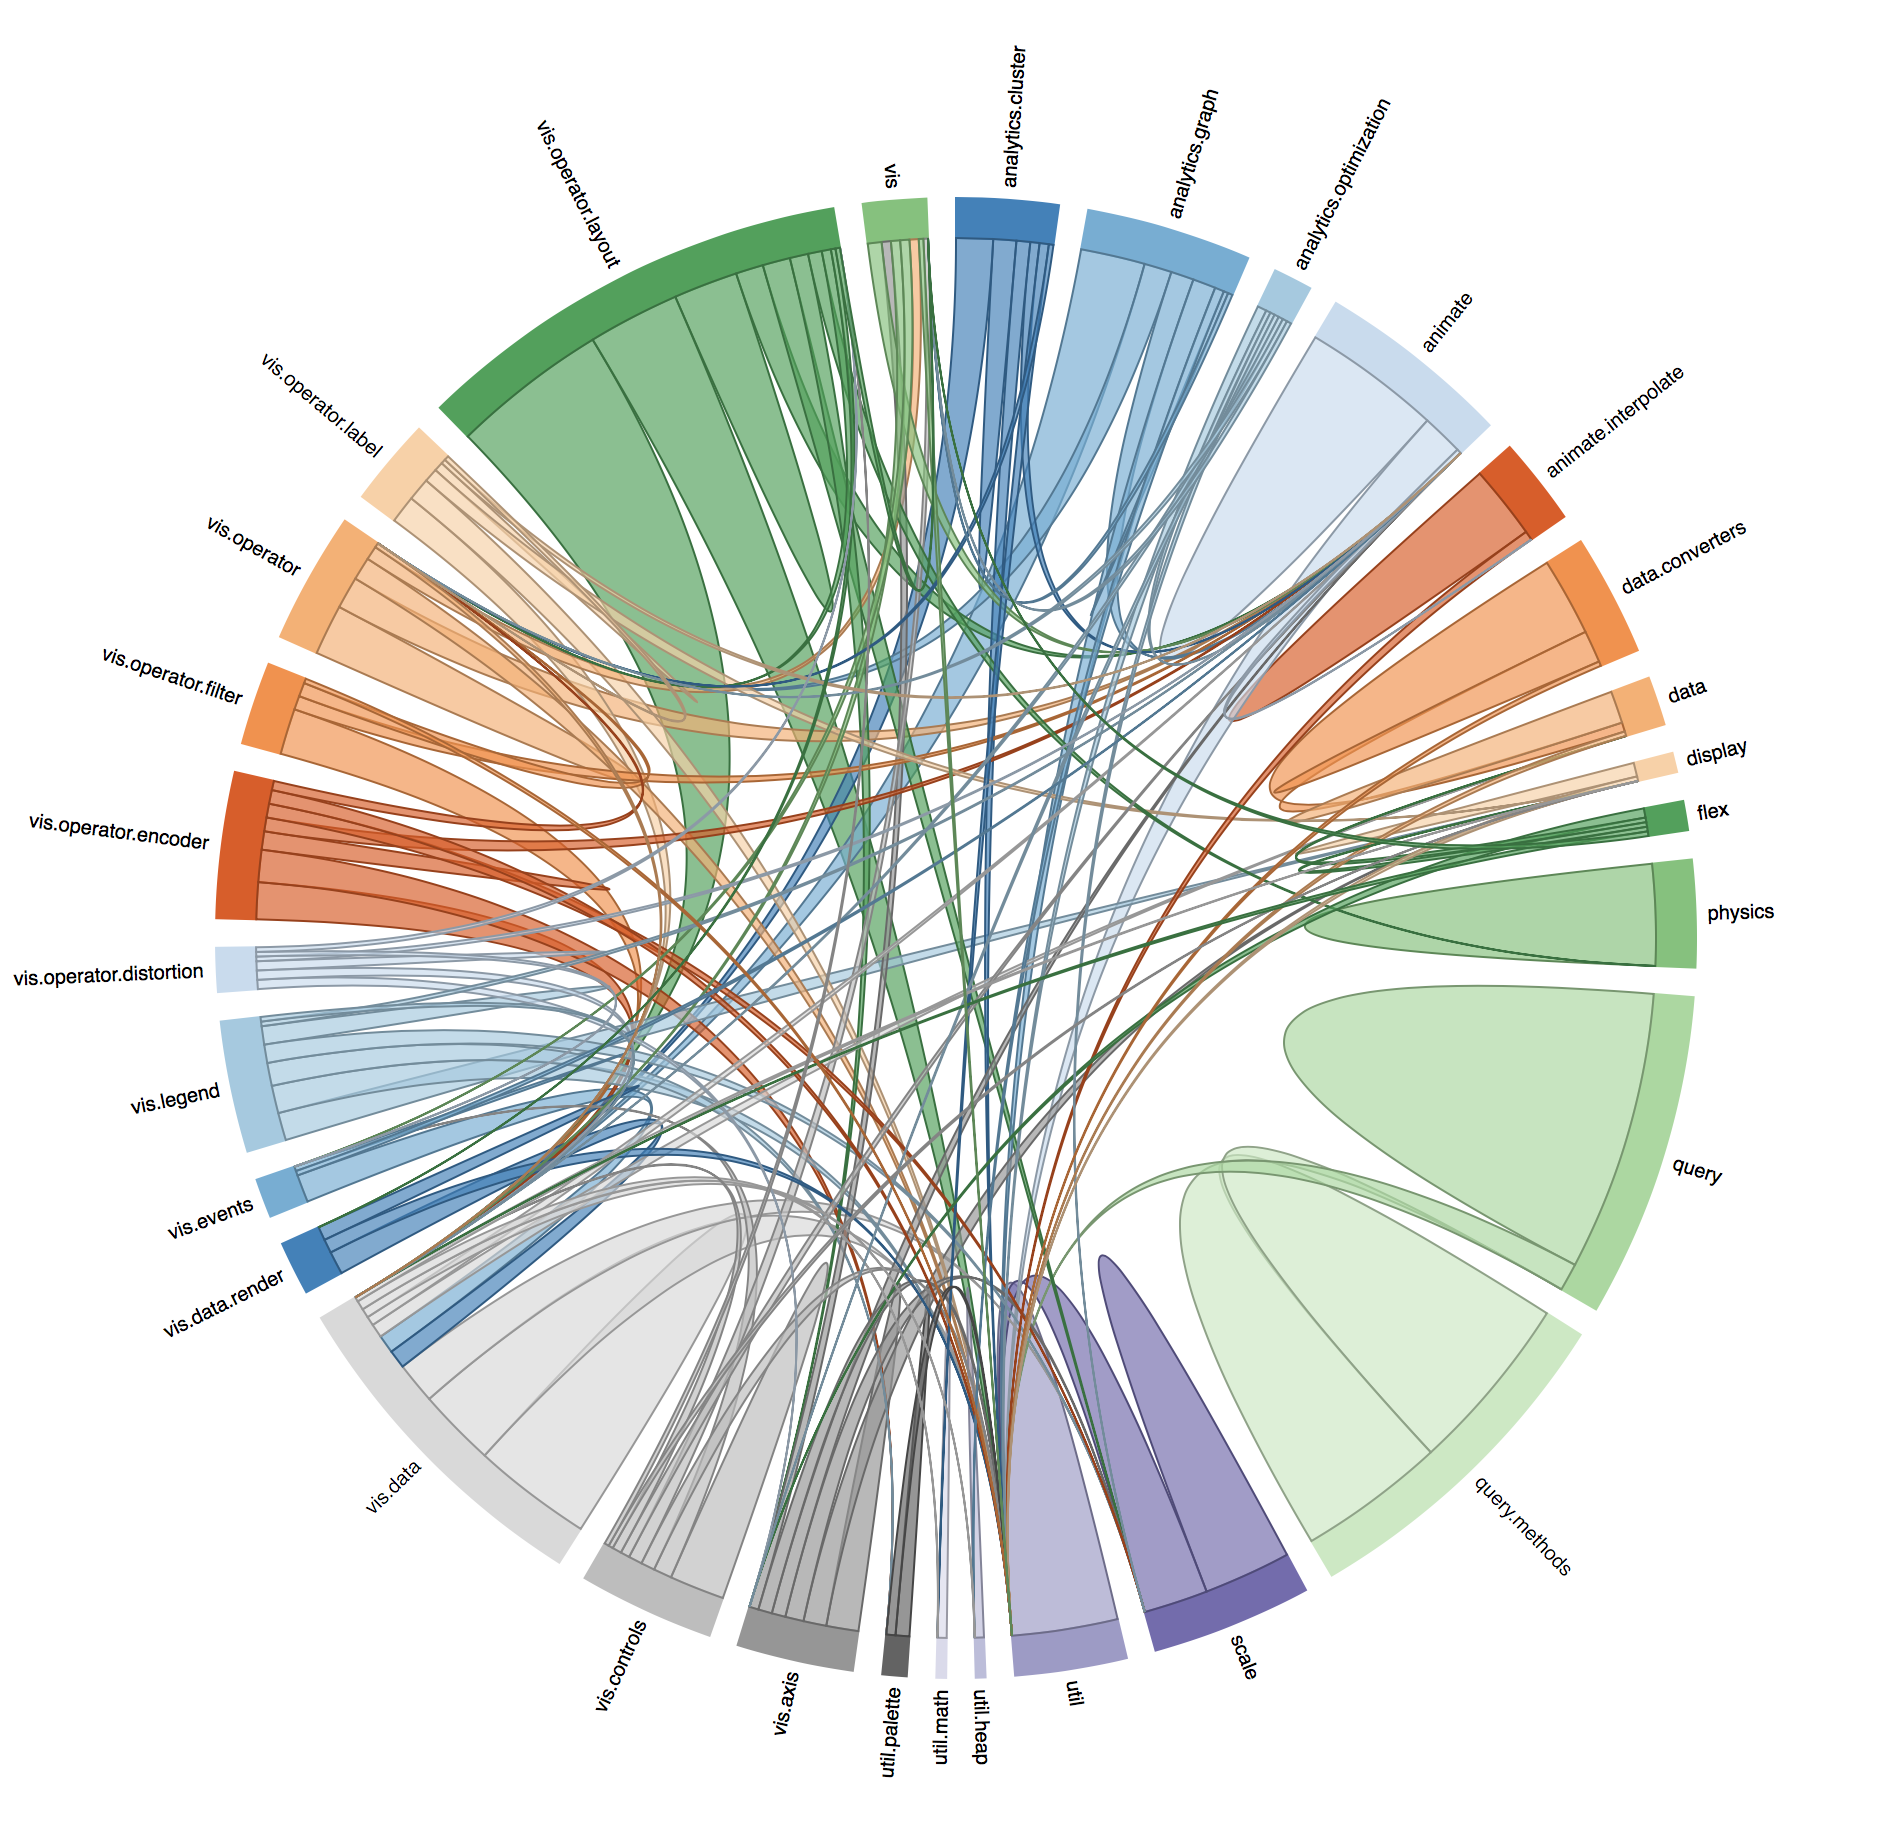
\includegraphics[width=8cm,keepaspectratio]{figures/fig13.png}
	\caption{\label{fig:13}A chord diagram using D3.js \citep{Bostock2017}.}
\end{figure}
	
	\item A tool to generate a sun-burst diagram for visualising multivariate data into sequential order, see Figure \ref{fig:14}

\begin{figure}[H]
	\centering
	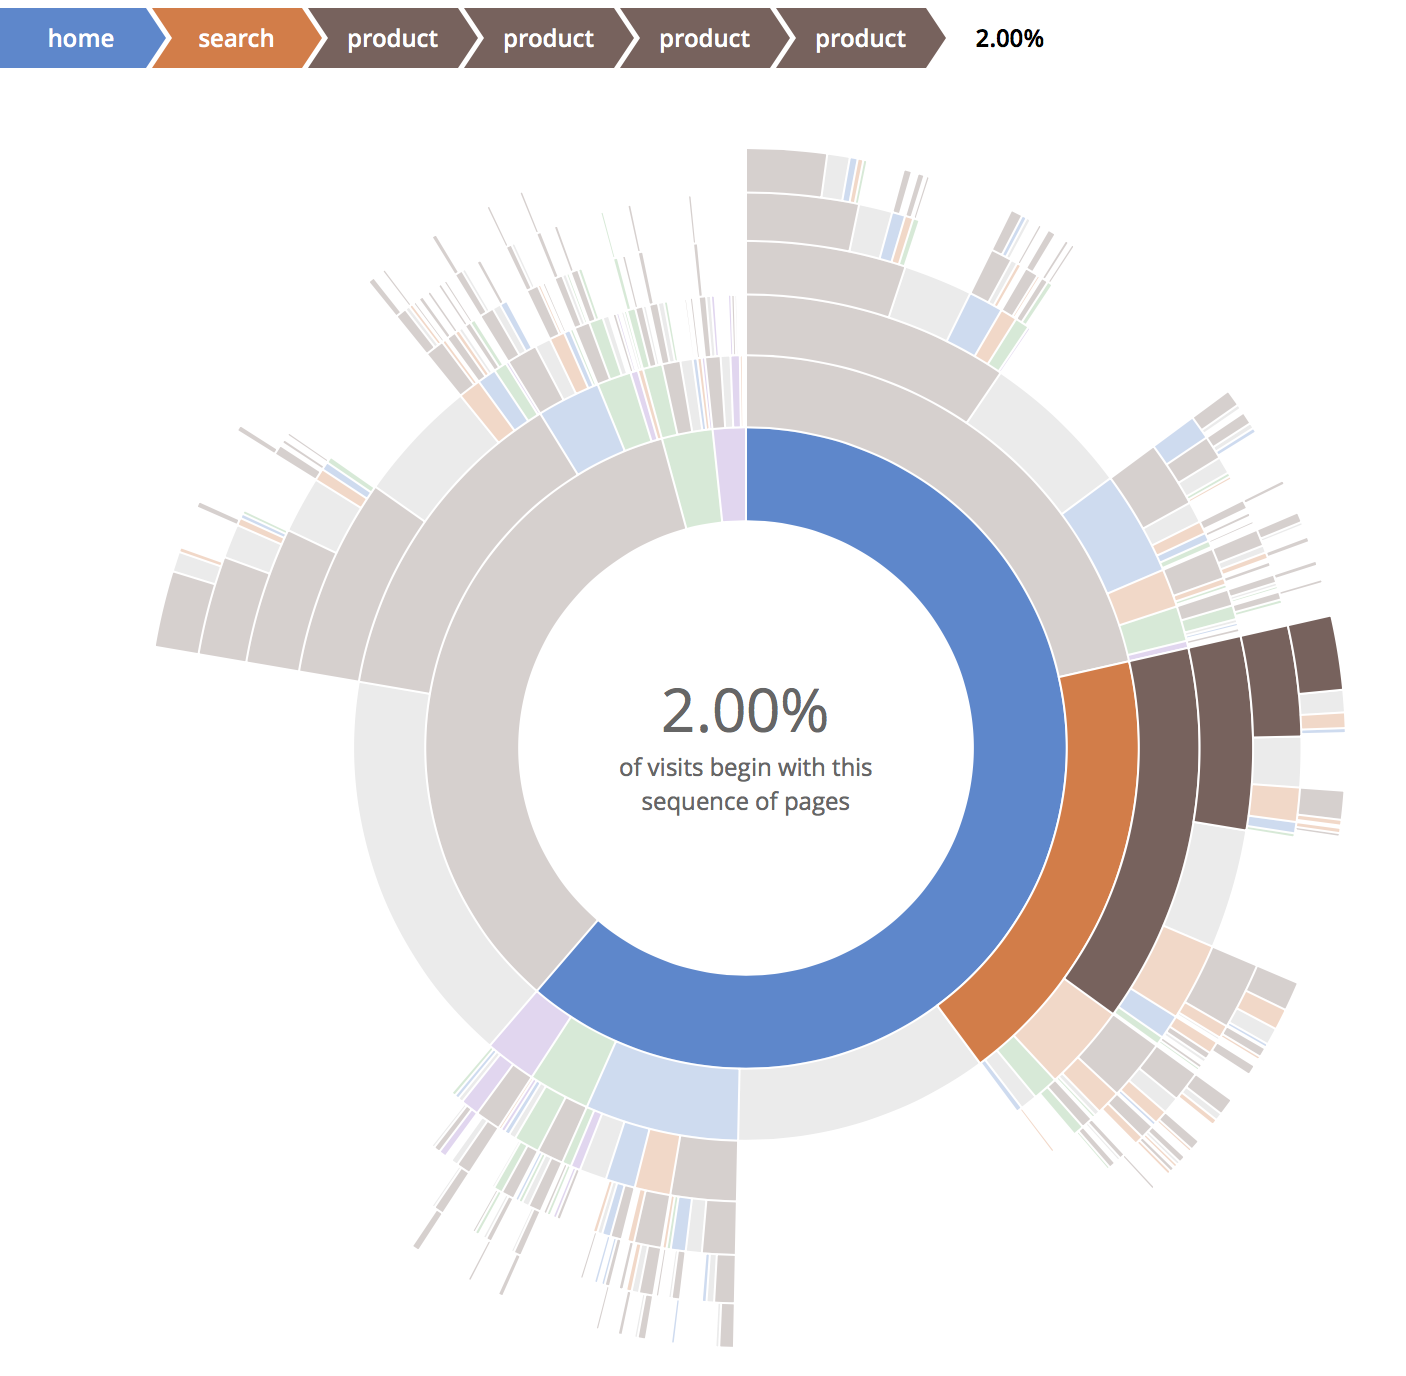
\includegraphics[width=8cm,keepaspectratio]{figures/fig14.png}
	\caption{\label{fig:14}A sun-burst diagram using D3.js \citep{Rodden2017}.}
\end{figure}
	\end{enumerate}
	\item A function to adjust time in order to present time-oriented data dimension
	\item A function to filter the data to be visualised
	\item A function to export the visualisation in image format

\end{enumerate}

\subsection{Technology Choices}
This section introduces the fundamental technology used, different technology will be used during different phase of the development, to suite the needs during the phase. 

The primary hardware for the development will be on a MacBook Pro embedded with an Intel i7-6920HQ CPU and 16GB of RAM, with the operating system of macOS Sierra 10.12.4. This will ensure that the large dataset can be pre-processed efficiently and the hardware is sufficient to run virtual machines of other operating system for testing purpose.
\subsubsection{Data Pre-processing}\hfil\newline
Java is chosen as the primary language for data pre-processing. Java is one of the most popular programming language that has great cross platform support with detailed documentation. The author also has years of experience in Java, thus Java is chosen to expedite the data pre-processing phase.

JSON-simple \citep{Fang} is a Java library that enables Java for manipulating JSON format in accordance with JSON specification RFC4627 \citep{JSON}. Taxi operational data in CSV is piped into Java program written for producing GeoJSON format follows the specification RFC7946 \citep{GeoJSON} that Mapbox Studio accepts.

The IDE for Java will be Eclipse version 4.6.3 with JDK build 1.8.0\_121\-b1.
\subsubsection{Web Application Development}\hfil\newline
The toolset will be presented in the form of Web application, all interactive functions will be manipulated by users via browsers. The application will mainly use HTML and CSS for presentation and JavaScript for functionality.

This combination is supported by any modern device with a screen, there are many existing frameworks such as AngularJS and Bootstrap to expedite the development process.

Microsoft Visual Studio IDE was considered to be the IDE for the development of Web Application. The IDE is fully-featured with development, testing and publication of the application. However, it only supports Windows and the publication and hosting of the application is tied to Windows Azure. Therefore, Microsoft Visual Studio Code, the code editor that inherits a certain level of functionality from the IDE, will be used for the development. 

\begin{figure}[H]
	\centering
	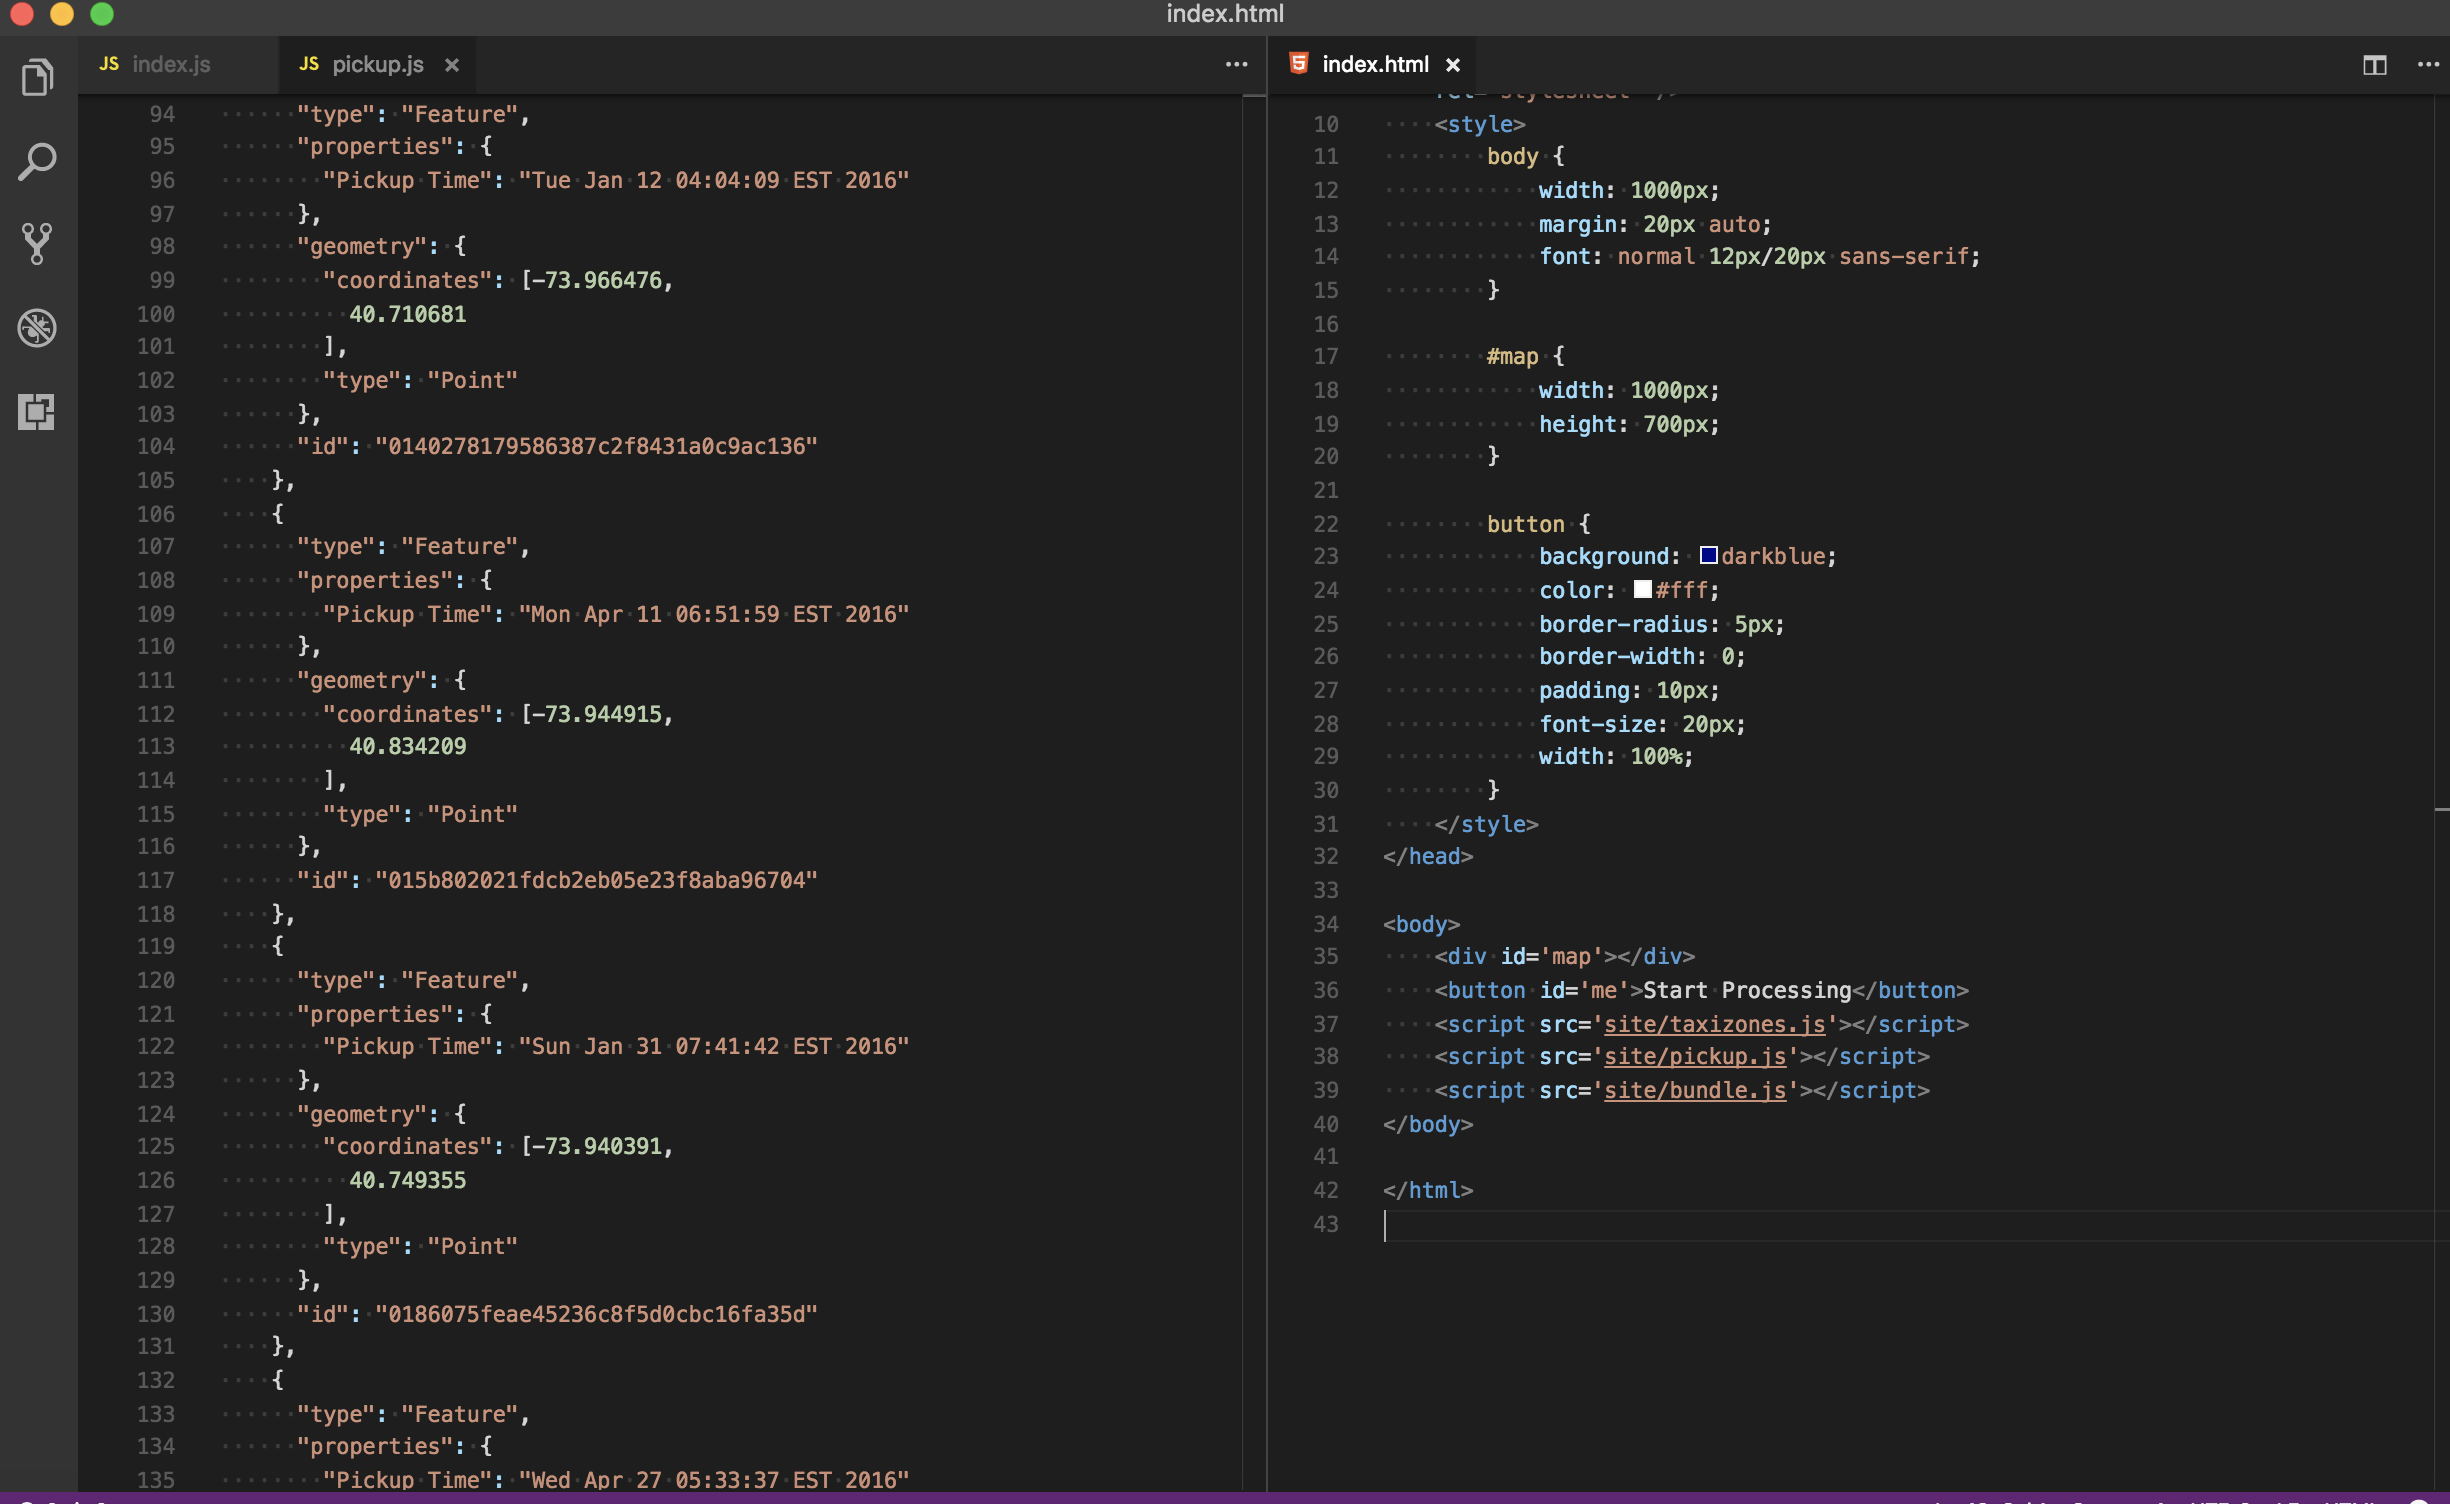
\includegraphics[width=\textwidth,keepaspectratio]{figures/fig16.png}
	\caption{\label{fig:16}Interface of Visual Studio Code editing HTML and JavaScript files. }
\end{figure}

Visual Studio Code is open source (MIT License) and has a huge library of extensions with active communities, it supports all major operating system. More importantly, it is capable of handling all the tasks involved in the development.

Visual Studio Code version 1.11.2 will be used for completing the web application.

\subsubsection{Others}\hfil\newline
\paragraph{Version Control System}\hfil\newline
Git is the most widely used version control system that is free (GNU General Public License v2) and supports all major operating systems. 

The free Git repository hosting service GitHub will be used to store all the code. GitHub will also serve as a regular backup warehouse to prevent any accident that may result in lost or corrupted files.

Git version 2.11.0 with the command line tools will be used throughout the whole development lifecycle.

\paragraph{Testing and Documentation}\hfil\newline
Testing and documentation are two essential steps for software development. According to Vliet, the cost of repairing errors made at an early stage is extremely high if they are discovered at a late stage of the development \citep[p. 386]{Vliet2007}, thus the testing should be frequently conducted during the development to minimise the negative impact of error and bugs.

Unit Testing is a testing process applied on every testable parts of a software, instead of testing the software as a whole, the focus of unit testing is the smaller building blocks called \textit{unit}, such as classes and procedures \citep[p. 85]{Myers2004a}. The benefits of unit testing are apparent:
\begin{itemize}
	\item Each unit and combinations of units are covered easily
	\item Reflecting impacts from code modifications
	\item Locating errors precisely to its source
\end{itemize}

JUnit is a framework to conduct unit testing for Java, Emma is an open source (Common Public License v1.0) JUnit tool for Eclipse \citep{Roubtsov2010}, it is capable of automating unit testing and will be used the development and testing stage of this project. Similarly, the parts of implementation using JavaScript will be unit tested using QUnit \citep{qunit}.

Doxygen \citep{Doxygen} will be used as the documentation generating tool, it is free under the GNU General Public License v2. Following Bob's Concise Introduction to Doxygen \citep{Laramee2011}, Doxygen is capable of generating well structured documents base on the comments in the code. It will also product class hierarchy and collaboration diagrams. A HTML version will also be generated, makes it easier to publish the documentation online.

Using Doxygen also encourages developer to comment the code during development, this improves code quality and reduces bugs.

\section{Project Plan and Timetable}
\label{sec4}
\subsection{Development Strategy}
\label{Development Strategy}

These are five essential stages of software development \citep[p .11]{Laramee2011a, Vliet2007}.

Five sections are included in the gantt chart:
\begin{enumerate}
	\item Requirements specification
	\item Software design
	\item Implementation
	\item Testing
	\item Documentation
\end{enumerate}

Requirements specification refers to 

Arnuphaptrairong \citep{Arnuphaptrairong2011} discovered that project planning is the area where the most number of risks originated. Therefore, this project will strictly adopt the Scrum Agile software development framework to plan and control the project development throughout the whole lifecycle.

\begin{figure}[H]
	\centering
	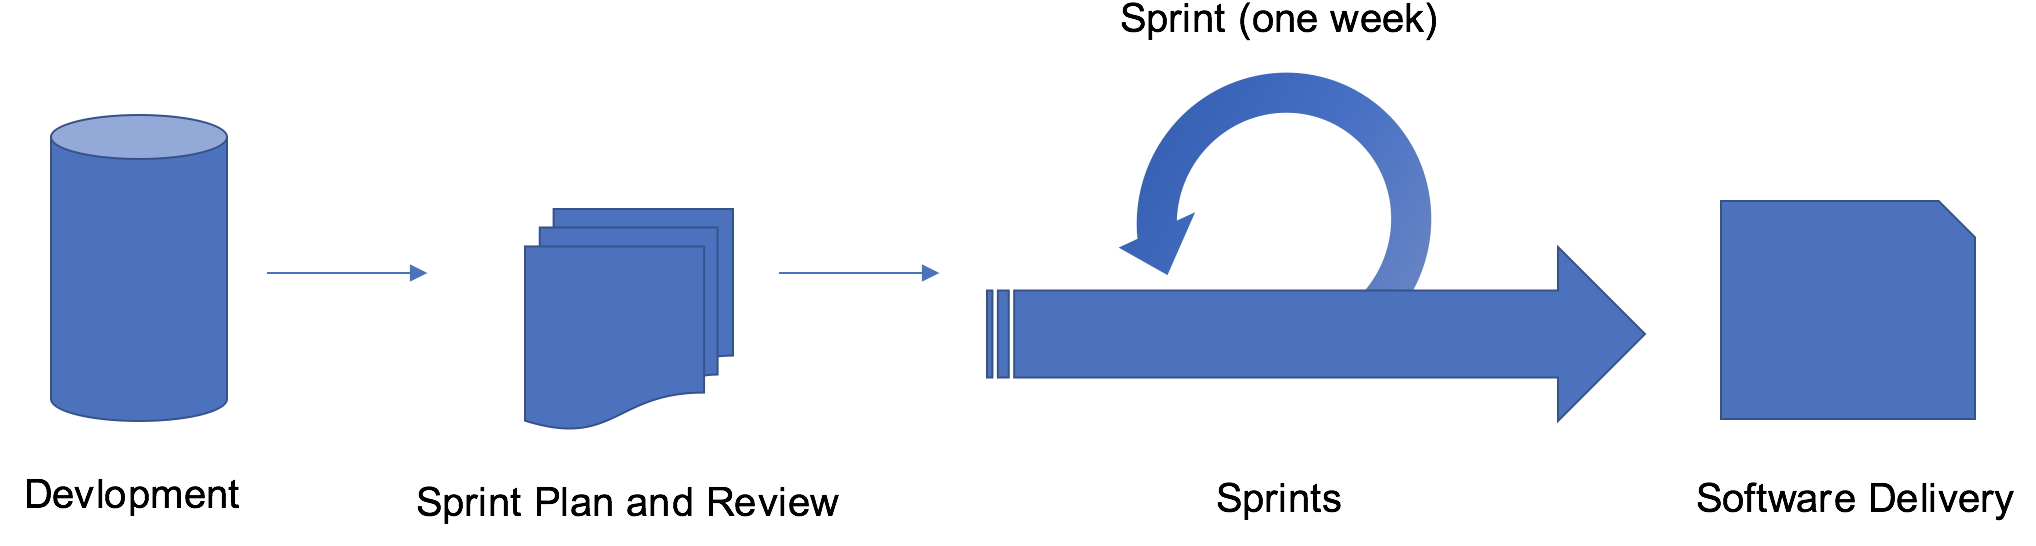
\includegraphics[width=\textwidth,keepaspectratio]{figures/fig15.png}
	\caption{\label{fig:15}Slightly modified Scrum workflow for this project. }
\end{figure}

Scrum is the most widely adopted Agile framework. Figure \ref{fig:15} shows a Scrum workflow tailored for this project. Development is broken into smaller Sprints, each Sprint takes one week to develop, completion of all Sprints signals the shipment of software. The original Scrum workflow requires a daily team meeting during each Spring, since the author is the only developer in the team, a daily meeting with team members during each Spring is cancelled. Sprint requires planning ahead and reviewing after, at the end of each Sprint, the development team will review it with stakeholders to identify improvements or corrections needed.

The flexibility of Scrum allows the author to embrace changes to requirements and correct misinterpretation of requirements within an acceptable timeframe.

\subsection{Gantt Chart}
Figure \ref{fig:ganttchart} shows the gantt chart for this project. 

\begin{sidewaysfigure}
\begin{figure}[H]
\definecolor{barblue}{RGB}{153,204,254}
\definecolor{groupblue}{RGB}{51,102,254}
\begin{ganttchart}[
            x unit=0.068cm,
            y unit title=0.7cm,
            y unit chart=0.8cm,
    time slot format=isodate,
    progress=today,
    time slot format/start date=2017-02-24, 
 	today={\the\year-\the\month-\the\day}, 
    title/.style={fill=teal, draw=none},
	title label font=\color{white}\bfseries,
    include title in canvas=false,
    bar label node/.append style={left=0.1cm},
    bar/.append style={fill=black!63},
    bar incomplete/.append style={fill=barblue},
    bar left shift=0.1,
    bar height=0.25,
    group incomplete/.append style={fill=groupblue},
    group left shift=0.1,
    group right shift=0,
    group height=0.25,
    group peaks tip position=0,
	group peaks height=0.4,
            bar label node/.style={align=left,font=\small\raggedleft,anchor=east},
            milestone label node/.style={align=left,font=\small\raggedleft,anchor=east},
            group label node/.style={align=left,font=\small\bfseries\raggedleft,anchor=east},    
            bar progress label node/.style={anchor=north, font=\scriptsize},
            group progress label node/.style={anchor=north, font=\scriptsize}
            ]{2017-02-24}{2017-09-30}
\gantttitlecalendar{month=shortname} \\
\ganttgroup[name=G1]{Requirements specification (76d)}{2017-02-24}{2017-05-11}\\
\ganttbar[name=T11]{Initial project presentation (18d)}{2017-02-24}{2017-03-14}\\
\ganttbar[name=T12]{Initial project specification (57d)}{2017-03-15}{2017-05-11}\\

\ganttgroup[name=G2]{Software design (61d)}{2017-04-12}{2017-06-12}\\
\ganttbar[name=T21]{Data pre-processing (48d)}{2017-04-12}{2017-05-30}\\
\ganttbar[name=T22]{Basic feature design (10d)}{2017-06-01}{2017-06-11}\\
\ganttbar[name=T23]{Advanced feature design (11d)}{2017-06-01}{2017-06-12}\\

\ganttgroup[name=G3]{Implementation (73d)}{2017-06-13}{2017-08-25}\\
\ganttbar[name=T31]{Basic feature implementation (63d)}{2017-06-13}{2017-08-15}\\
\ganttbar[name=T32]{Advanced feature implementation (10d)}{2017-08-15}{2017-08-25}\\

\ganttgroup[name=G4]{Testing (28d)}{2017-8-28}{2017-9-25}\\
\ganttbar[name=T41]{Testing (20d)}{2017-08-28}{2017-09-17}\\
\ganttbar[name=T42]{Bug fixes (13d)}{2017-09-12}{2017-09-25}\\

\ganttgroup[name=G5]{Documentation (5d)}{2017-09-25}{2017-09-30}\\
\ganttbar[name=T51]{Doxygen (5d)}{2017-09-25}{2017-09-30}\\
\ganttbar[name=T52]{Review (5d)}{2017-09-25}{2017-09-30}\\

\ganttlink{T11}{T12}
\ganttlink{T12}{T21}
\ganttlink{T21}{T22}
\ganttlink{T22}{T31}
\ganttlink{T31}{T41}
\ganttlink{T42}{T51}
\end{ganttchart}
	\caption{\label{fig:ganttchart}Project gantt chart as of \today}
\end{figure}	
\end{sidewaysfigure}

%\begin{figure}
%\definecolor{barblue}{RGB}{153,204,254}
%\definecolor{groupblue}{RGB}{51,102,254}
%\begin{ganttchart}[
%    hgrid,
%    vgrid,
%            x unit=0.05cm,
%            y unit title=0.7cm,
%            y unit chart=1.15cm,
%    time slot format=isodate,
%    progress=today,
%    time slot format/start date=2017-02-24, 
% 	today={\the\year-\the\month-\the\day}, 
%    title/.style={fill=teal, draw=none},
%	title label font=\color{white}\bfseries,
%    include title in canvas=false,
%    bar label node/.append style={left=0.1cm},
%    bar/.append style={fill=black!63},
%    bar incomplete/.append style={fill=barblue},
%    bar left shift=0.1,
%    bar height=0.25,
%    group incomplete/.append style={fill=groupblue},
%    group left shift=0.1,
%    group right shift=0,
%    group height=0.25,
%    group peaks tip position=0,
%	group peaks height=0.4,
%            bar label node/.style={text width=3cm,align=left,font=\small\raggedleft,anchor=east},
%            milestone label node/.style={text width=2cm,align=left,font=\small\raggedleft,anchor=east},
%            group label node/.style={text width=3cm,align=left,font=\small\bfseries\raggedleft,anchor=east},    
%            bar progress label node/.style={text width=3cm,anchor=north, font=\scriptsize},
%            group progress label node/.style={text width=3cm,anchor=north, font=\scriptsize}
%            ]{2017-02-24}{2017-09-30}
%\gantttitlecalendar{month=shortname} \\
%\ganttgroup[name=G1]{Requirements specification (76d)}{2017-02-24}{2017-05-11}\\
%\ganttbar[name=T11]{Initial project presentation (18d)}{2017-02-24}{2017-03-14}\\
%\ganttbar[name=T12]{Initial project specification (57d)}{2017-03-15}{2017-05-11}\\
%
%\ganttgroup[name=G2]{Software design (61d)}{2017-04-12}{2017-06-12}\\
%\ganttbar[name=T21]{Data pre-processing (48d)}{2017-04-12}{2017-05-30}\\
%\ganttbar[name=T22]{Basic feature design (10d)}{2017-06-01}{2017-06-11}\\
%\ganttbar[name=T23]{Advanced feature design (11d)}{2017-06-01}{2017-06-12}\\
%
%\ganttgroup[name=G3]{Implementation (73d)}{2017-06-13}{2017-08-25}\\
%\ganttbar[name=T31]{Basic feature implementation (63d)}{2017-06-13}{2017-08-15}\\
%\ganttbar[name=T32]{Advanced feature implementation (10d)}{2017-08-15}{2017-08-25}\\
%
%\ganttgroup[name=G4]{Testing (28d)}{2017-8-28}{2017-9-25}\\
%\ganttbar[name=T41]{Testing (20d)}{2017-08-28}{2017-09-17}\\
%\ganttbar[name=T42]{Bug fixes (13d)}{2017-09-12}{2017-09-25}\\
%
%\ganttgroup[name=G5]{Documentation (5d)}{2017-09-25}{2017-09-30}\\
%\ganttbar[name=T51]{Doxygen (5d)}{2017-09-25}{2017-09-30}\\
%\ganttbar[name=T52]{Review (5d)}{2017-09-25}{2017-09-30}\\
%
%\ganttlink{T11}{T12}
%\ganttlink{T12}{T21}
%\ganttlink{T21}{T22}
%\ganttlink{T22}{T31}
%\ganttlink{T31}{T41}
%\ganttlink{T42}{T51}
%\end{ganttchart}
%	\caption{\label{fig:ganttchart}Project gantt chart as of \today}
%\end{figure}

\subsection{Risk Analysis}
This analysis outlines the potential risks that will have catastrophic damage on the development or severely affect the progress of development and strategies to counter them. 

\subsubsection{Risk Identification}\hfil\newline
The identification of risks followed the research carried out by Arnuphaptrairong \citep{Arnuphaptrairong2011}. Seven risks are rated as the most frequently encountered in software development lifecycle in the research as follows:
\begin{enumerate}
	\item Misunderstanding of requirements
	\item Lack of top management commitment and support
	\item Lack of adequate user involvement
	\item Failure to gain user commitment
	\item Failure to manage end user expectation
	\item Changes to requirements
	\item Lack of an effective project management methodology
\end{enumerate}

\subsubsection{Risk Mitigation}\hfil\newline
This section outlines the mitigation measures against the risks identified.

Table \ref{tab:4} shows the risk identified by the author. The first risk, the involvement of new technology with high level of technical complexity is rated as the riskiest factor. Obstacles are expected in the project due to the novelty of the author, the involved technology will be carefully selected by the following factors:
\begin{itemize}
	\item Language structure and syntax are close to the author's prior experience  
	\item Detailed documentation for the technology 
	\item Preferably free and open source 
	\item Active communities are in place
	\item Successful software built upon the technology can be accessed and reviewed
\end{itemize}

The second risk, misinterpretation of requirements has serious consequence, it mitigated by conducting regular meeting with supervisor. Scrum workflow also helps minimise the risk.

The third risk, Java and JavaScript are the main languages used for this project, they are both well-documented and have active communities to provide technical support. This mitigates the risk from inadequate programming skills of the author.

\begin{table}[H]
	\centering
			\caption{Risk analysis and mitigation}
	\label{tab:4}
	\begin{tabularx}{\textwidth}{p{0.2cm} X|>{\raggedleft\arraybackslash}p{2cm}|>{\raggedleft\arraybackslash}p{1.2cm}|X}
		\hline\hline
		& \textbf{Risk} & \textbf{Probability} & \textbf{Impact} & \textbf{Mitigation measures} \\\hline
		1&	Involvement of new technology with high level of technical complexity & High & High & Choose the technology involved carefully, avoid unrealistic or unnecessary features and invest more time into exploring the technology	used	 \\\hline
		2&Misinterpretation of requirements                      & Medium            & High            &  Regular meeting with supervisor for consultations and progress monitoring     \\\hline
		3&Inadequate skills and knowledge in programming        & Medium             & High         &    Experienced programming language with detailed documentation and active community is used   \\\hline
		4&The final software developed has serious bugs that makes it unusable & Medium & High  & Features are developed in an order ranked by their value/risk ratio \\\hline
		5&Insufficient user involvement and feedback                   & Medium        &    Medium        &   Volunteers with data visualisation background are regularly surveyed when each version rolls out     \\\hline
		6&Equipment failure resulting in loss of files & Low & High & GitHub and Dropbox are used for regular backup of files. Laptop is backup daily using an external harddrive 	\\\hline
		7&Lack of effective project management skill & Low & High & Adopt Scrum Agile software development framework strictly 	\\\hline
		8&Personal illness  & Low & Medium & GP Surgeries are within reach\\\hline
		\hline
	\end{tabularx}
\end{table}

The fourth risk,  the development will start with high-value features with low-risk, proceeding to low-value features with low-risk and eliminating or substituting low-value features with high-risk. This ensures that the final project will deliver useable features.

The fifth risk, two volunteers with Data Visualisation background are chosen to test the features at the end of each or several Sprints, provide insightful feedback to minimise the risk brought by insufficient user involvement and feedback.

The sixth risk, GitHub, Dropbox and a local external harddrive are used for backup to ensure any equipment failure will not result in delay of the development.

The seventh risk, lack of effective project management skill, is mitigated by adopting Scrum Agile software development framework mentioned in \hyperref[Development Strategy]{Second 4.1 Development Strategy}.

The last risk is personal illness which is unavoidable, ensuring GP Surgeries are within reach can help minimise the damage.

\section{Initial Implementation}
\label{sec5}
\subsection{Data Pre-processing}

\subsection{Implementation}


\cleardoublepage
\bibliographystyle{apalike}
\bibliography{sc}
\end{document}